\section{Ukázková kapitola}

\subsection{Struktura a formát}

\subsubsection{Jak strukturovat práci}



Práci strukturujte tak, abyste měli několik hlavních kapitol (ideálně méně než 10), jednotlivé kapitoly dělte do podkapitol maximálně do třetí úrovně. U~bakalářských a~diplomových prací se více úrovní považuje za problém se strukturováním myšlenek.

Kapitoly první úrovně vždy začínají na nové stránce (ostatní úrovně nikoliv). To je nastaveno ve stylu, nemusíme se o nic starat. Do nadpisů kapitol nedáváme závorky. Pokud chceme použít zkratku a zároveň ji vysvětlit, neprovádíme to v~nadpisu, ale třeba v prvním odstavci.

Neměla by nastat situace, kdy hned za některým nadpisem následuje seznam, obrázek, tabulka či jiný podobný útvar. Vždy by před něčím takovým měla být vysvětlující \uv{omáčka}, alespoň jedna věta.



\subsection{Obrázky a tabulky}


Obrázky a~tabulky mají být uzavřeny v příslušném prostředí (pro obrázky je to \uv{figure}, pro tabulky \uv{table}, vždy s titulkem, viz níže). Toto prostředí zajistí správné zarovnání a umístění objektu. Není nutné, aby objekt byl přesně na místě, kde se o něm píše v textu, lze použít odkaz, třeba na obrázek \ref{fig:slecnasnotebookem} na straně \pageref{fig:slecnasnotebookem}.

Popisky sázíme pod obrázky a~nad tabulky. Popisek nebastlete ručně, ale využijte prostředky \LaTeX u -- důvodem je, aby bylo možné automaticky vygenerovat seznam obrázků a~seznam tabulek.

\begin{figure}[htb]
	\centering
		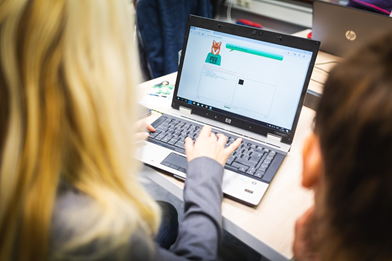
\includegraphics[width=.5\textwidth]{slecna-s-notebookem.png}
	\caption[Ukázka vložení titulku s~označením zdroje]{Ukázka vložení titulku s~označením zdroje\cite{mytyprog}}
	\label{fig:slecnasnotebookem}
\end{figure}


Všimněte si ve zdroji souboru (v~tomto případě soubor zakladni-info.tex), jak je zajištěno, aby označení zdroje sice bylo u~obrázku, ale neobjevilo se v~seznamu obrázků -- makro \ttsmall{\zpetnelomitko{}caption} má povinný parametr (to, co se objeví u~obrázku) i~nepovinný parametr (to, co se objeví v~seznamu obrázků).

V~tabulkách použijte raději řádkování trochu užší než 1,5, třeba 1.1 nebo 1.2.

Pokud jste přejali tabulku nebo to, co se v~ní nachází, také je nutné uvést zdroj, podobně jako u~obrázku.

Pokud obrázky a~tabulky nepoužíváte (nebo máte jednu či dvě), vzadu odstraňte seznam obrázků/tabulek.


\begin{table}[htb]
	\centering
	\caption{Ukázka tabulky}
	\medskip
	\radkovani[1.2]
		\begin{tabular}{@{}l||l|c|c@{}}\hline
			\textbf{Číslo} & \textbf{Jméno} & \textbf{Věk} & \textbf{Očkování}\\ \hline\hline
			1	&Žeryk&	4	&ano\\ \hline
			2	&Andy&	7	&ano\\ \hline
			3	&Ťapka&	2	&ne\\ \hline			
		\end{tabular}
	\label{tab:ukazkatabulky}
\end{table}


\subsubsection{Vkládání ukázkového kódu}

Pokud vkládáte ukázkový kód, můžete buď formátovat ručně, nebo použít zde definované prostředí \ttsmall{prog}, nebo použít vhodný balíček, můžu doporučit například algorithm2e -- informace, manuál a~samotný balíček najdete na \cite{algorithm2e}.

Doporučení pro ruční formátování:
\begin{citemize}
	\item V~daném úseku nastavte řádkování na 1 nebo jen mírně větší:\\	
	\ttsmall{\zpetnelomitko radkovani[1]}
	
	\item Použijte neproporcionální písmo a~menší font:\\	
	\ttsmall{\{\zpetnelomitko ttfamily\zpetnelomitko small}\\[-2pt]
	\ttsmall{...}\\[-2pt]
	\ttsmall{\}}
	\item Vraťte řádkování na výchozí hodnotu:\\	
	\ttsmall{\zpetnelomitko radkovani}
\end{citemize}
Ukázka využití prostředí \ttsmall{prog}:

\begin{prog}
if (pocet_bodu > 100) {
	print ("chyba při výpočtu bodů nebo zásah hackera");
	ukonci_program();
}
if (pocet_bodu > 50)
	udelit_zapocet(pocet_bodu);
else
	informuj_nahradni_terminy();
\end{prog}

Kolem tohoto prostředí vždy nechejte volný řádek.



\subsection{Vyznačování pojmů v~textu}

Pokud potřebujeme v~textu vyznačit pojem, například tam, kde tento pojem vysvětlujeme, použijeme \emph{kurzívu}. Tučné písmo je vyhrazeno pro nadpisy a~pojmy v~glosáři, případně záhlaví tabulek, v~textu se nepoužívá.



\subsection{Odrážky, číslování, pojmenované odstavce}

Kapitoly první úrovně vždy začínají na nové stránce (ostatní úrovně nikoliv). To je nastaveno ve stylu, nemusíme se o~nic starat.

Před jakýmkoliv seznamem by měla být \uv{omáčková} věta či odstavec. Určitě nedávejte seznam hned pod nadpis, vždy před něj dopište nějaký text.

Odrážky vypadají takto:
\begin{citemize}
	\item první odrážka,
	\item druhá odrážka.
\end{citemize}
Případně si drobně upravte odsazení, prostředí je definováno v~souboru s~příponou .\textsc{cfg}.

Číslovaný sezinam vypadá následovně:
\begin{cenumerate}
	\item Odrážkové nebo číslované seznamy můžete pojmout jako součásti věty (pak položky končí čárkou, poslední tečkou, začínají malými písmeny).
	\item Druhá možnost je pojmout je jako samostatné věty, pak samozřejmě začínají velkým písmenem a~končí tečkou.
\end{cenumerate}

Finální úpravou je zajištění toho, aby na koncích řádků nebyly jednopísmenné předložky a~spojky. V~\LaTeX u~toho docílíme tak, že mezeru mezi jednopísmennou předložkou/spojkou a~následujícím slovem nahradíme vlnkou: \vlnka{}. Koncem řádku by taktéž nemělo být odděleno číslo od jednotky, tedy například 12~kg. Lze použít program \ttsmall{vlna} od Olšáka, informace a~program na \cite{vlnazdroj}.

Poznámky pod čarou používejte jen v~nejnutnějších případech -- prosím nenuťte čtenáře každou chvíli šilhat na konec stránky :-).

\paragraph{Pojmenovaný odstavec.} Takto můžete vyřešit situaci, kdy potřebujete sekci rozdělit, ale nechcete použít číslovaný nadpis (třeba proto, že tento text by byl jen krátký a~nemá smysl navážet ho do obsahu).

\paragraph{Když nemám editor.} Pokud nemáte nainstalován \LaTeX, můžete použít cloudovou variantu (dostupnou zdarma): \emph{Overleaf}. Vše potřebné najdete na \cite{overleaf}. Nebo si můžete nainstalovat třeba \MikTeX\cite{miktex}.



